\documentclass[11pt,a4paper,twoside,openright,bibliography=totoc]{scrbook}

\usepackage{scrhack}
\usepackage{graphicx,xcolor,float}
\usepackage{amssymb,amsmath,array}
\usepackage{setspace,algpseudocode}

\usepackage{tikz}
\usetikzlibrary{positioning,arrows,calc,intersections}

% Color citation, references and links.
\usepackage{url,hyperref}
\hypersetup{
  colorlinks,
  linkcolor={black},
  citecolor={red!70!black},
  urlcolor={blue!70!black}
}
\usepackage[labelfont=bf]{caption} % Bold figure titles.

\renewcommand{\t}{\text} % Shorten \text command.

\begin{document}
% Example of title page for the projects carried out within the lasec 

% Simply include it in your mastex tex file: 
%        % Example of title page for the projects carried out within the lasec 

% Simply include it in your mastex tex file: 
%        % Example of title page for the projects carried out within the lasec 

% Simply include it in your mastex tex file: 
%        \input{cover}


% Updated March 2006 (SP)


\newcommand{\logoepfl}[0]{
  \begin{center}
    
\includegraphics[width=4cm]{cover/logo_epfl_coul.eps}
  \end{center}
  \vspace{0.3cm}
  \hrule
}
\newcommand{\logolasec}[0]{
  \vspace{1cm}
  \hrule
  \begin{center}
    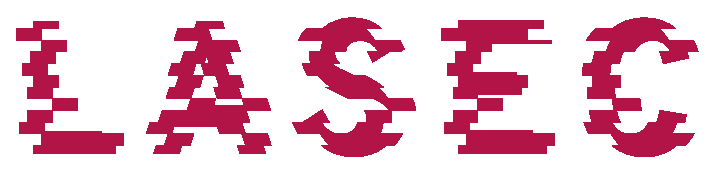
\includegraphics[width=4.5cm]{cover/logo_lasec_coul.eps}
  \end{center}
}
\newcommand{\project}[1]{
  \begin{center}
    \large{#1}
  \end{center}
  \vspace{1cm}
}
\newcommand{\department}[1]{
  \begin{center}
    \large{#1}
  \end{center}
}
\newcommand{\supervisor}[3]{
  \begin{center}
    \begin{normalsize}{
        \bfseries #1}\\#2\\#3
    \end{normalsize}
  \end{center}
}
\renewcommand{\author}[1]{
  \begin{center}
    \Large{#1}
  \end{center}
  \vspace{0.5cm}
}
\renewcommand{\title}[1]{
  \vspace{3cm}
  \begin{center}
    \huge{#1}
  \end{center}
  \vspace{1.7cm}
}
\renewcommand{\date}[2]{
  \begin{center}
    \normalsize{#1 #2}
  \end{center}
  \vspace{0.5cm}
}


\thispagestyle{empty}


% begin title page
\logoepfl

\title{Ratcheting}

\author{Andrea Caforio}
\department{School of Computer and Communication Sciences}
\project{Optional Semester Project}

\date{January}{2019}

\begin{center}
  \begin{tabular}{cc}
    \begin{tabular}{p{4.0cm}}
      \supervisor{Responsible}{Prof. Serge Vaudenay}{EPFL / LASEC}
    \end{tabular}&
    \begin{tabular}{p{4.0cm}}
      \supervisor{Supervisor}{Dr. Betül Durak}{EPFL / LASEC}
    \end{tabular}
  \end{tabular}
\end{center}

\logolasec
% end title page




% Updated March 2006 (SP)


\newcommand{\logoepfl}[0]{
  \begin{center}
    
\includegraphics[width=4cm]{cover/logo_epfl_coul.eps}
  \end{center}
  \vspace{0.3cm}
  \hrule
}
\newcommand{\logolasec}[0]{
  \vspace{1cm}
  \hrule
  \begin{center}
    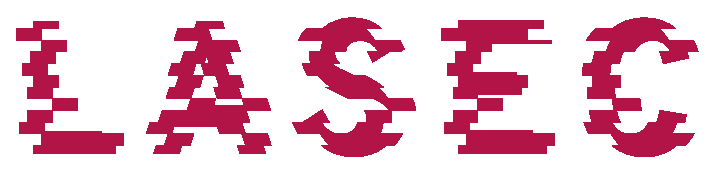
\includegraphics[width=4.5cm]{cover/logo_lasec_coul.eps}
  \end{center}
}
\newcommand{\project}[1]{
  \begin{center}
    \large{#1}
  \end{center}
  \vspace{1cm}
}
\newcommand{\department}[1]{
  \begin{center}
    \large{#1}
  \end{center}
}
\newcommand{\supervisor}[3]{
  \begin{center}
    \begin{normalsize}{
        \bfseries #1}\\#2\\#3
    \end{normalsize}
  \end{center}
}
\renewcommand{\author}[1]{
  \begin{center}
    \Large{#1}
  \end{center}
  \vspace{0.5cm}
}
\renewcommand{\title}[1]{
  \vspace{3cm}
  \begin{center}
    \huge{#1}
  \end{center}
  \vspace{1.7cm}
}
\renewcommand{\date}[2]{
  \begin{center}
    \normalsize{#1 #2}
  \end{center}
  \vspace{0.5cm}
}


\thispagestyle{empty}


% begin title page
\logoepfl

\title{Ratcheting}

\author{Andrea Caforio}
\department{School of Computer and Communication Sciences}
\project{Optional Semester Project}

\date{January}{2019}

\begin{center}
  \begin{tabular}{cc}
    \begin{tabular}{p{4.0cm}}
      \supervisor{Responsible}{Prof. Serge Vaudenay}{EPFL / LASEC}
    \end{tabular}&
    \begin{tabular}{p{4.0cm}}
      \supervisor{Supervisor}{Dr. Betül Durak}{EPFL / LASEC}
    \end{tabular}
  \end{tabular}
\end{center}

\logolasec
% end title page




% Updated March 2006 (SP)


\newcommand{\logoepfl}[0]{
  \begin{center}
    
\includegraphics[width=4cm]{cover/logo_epfl_coul.eps}
  \end{center}
  \vspace{0.3cm}
  \hrule
}
\newcommand{\logolasec}[0]{
  \vspace{1cm}
  \hrule
  \begin{center}
    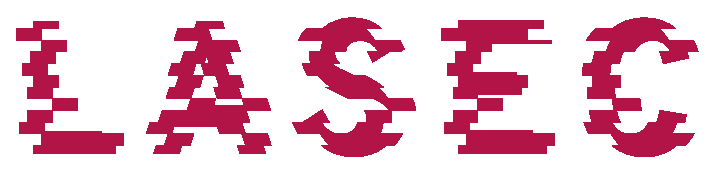
\includegraphics[width=4.5cm]{cover/logo_lasec_coul.eps}
  \end{center}
}
\newcommand{\project}[1]{
  \begin{center}
    \large{#1}
  \end{center}
  \vspace{1cm}
}
\newcommand{\department}[1]{
  \begin{center}
    \large{#1}
  \end{center}
}
\newcommand{\supervisor}[3]{
  \begin{center}
    \begin{normalsize}{
        \bfseries #1}\\#2\\#3
    \end{normalsize}
  \end{center}
}
\renewcommand{\author}[1]{
  \begin{center}
    \Large{#1}
  \end{center}
  \vspace{0.5cm}
}
\renewcommand{\title}[1]{
  \vspace{3cm}
  \begin{center}
    \huge{#1}
  \end{center}
  \vspace{1.7cm}
}
\renewcommand{\date}[2]{
  \begin{center}
    \normalsize{#1 #2}
  \end{center}
  \vspace{0.5cm}
}


\thispagestyle{empty}


% begin title page
\logoepfl

\title{Ratcheting}

\author{Andrea Caforio}
\department{School of Computer and Communication Sciences}
\project{Optional Semester Project}

\date{January}{2019}

\begin{center}
  \begin{tabular}{cc}
    \begin{tabular}{p{4.0cm}}
      \supervisor{Responsible}{Prof. Serge Vaudenay}{EPFL / LASEC}
    \end{tabular}&
    \begin{tabular}{p{4.0cm}}
      \supervisor{Supervisor}{Dr. Betül Durak}{EPFL / LASEC}
    \end{tabular}
  \end{tabular}
\end{center}

\logolasec
% end title page


\tableofcontents

\chapter{Introduction}
\label{chap:introduction}

Messaging has become an ubiquitous resource in the daily lives of
millions of people around the globe through the widespread adoption of
instant messaging applications. The design of protocols which
facilitate securing messaging or key-agreement is faced with a unique
set of challenges, this is due to the longevity of sessions between
communicating parties and the inherently asynchronous notion of
messaging where a participant is both the sender and recipient of
messages and the time a message is sent or received is undefined. In
such a setting the leakage of a state to the adversary is especially
devastating since in a naive protocol it would not only enable him to
recover past messages but also allow future impersonations of the
victim.
Ratcheting has established itself as the go-to technique in
order to mitigate these risks. Akin to its mechanical equivalent the
states are continuously moved forward (updated) without the
possibility of going backwards, i.e.~it should be impossible to
recover past states from the current one.
\begin{figure}[h]
  \centering
  
\includegraphics[scale=0.1]{figures/ratchet-icon.eps}
  \caption[Symbolic Ratchet Wheel]{Symbolic Ratchet Wheel\footnotemark}
  \label{fig:ratchet-wheel}
\end{figure}
\footnotetext{\url{https://www.iconfinder.com/icons/328526}}
This further implies that
past message remain secure even in the presence of and adversary who
can expose the state of a participant. The literature labels protocols
that deploy ratchets as \textit{forward-secure}. This technique saw
its inception in 2004 as part of the Off-the-Record messaging
protocol~\cite{borisov2004off}. It only recently gained traction
through the massively popular Signal protocol~\cite{perrin2016double}.
The release of this protocol however predates its first formal
security analysis in 2017~\cite{cohn2017formal}
and since then several novel protocols with various degrees of
security levels have been proposed. Among others
these protocols also attempt the satisfy the notion of \textit{future
secrecy} in which future states and messages remain secure even if the
current state has been leaked. Furthermore, a secure messaging
protocol should be efficient enough to run smoothly even on
computationally inferior devices thus the choice of fast primitives
that do not compromise the promised security levels play a crucial
part in the construction of messaging protocols. Even though on paper
the attained levels of security in these new protocol often only
differ marginally the effects on performance metrics are of a
different kind with sometimes huge differences between the protocols.

% Add some more text here.

\section{Contributions}
\label{sec:contributions}

This project is concerned with surveying and solidifying the
performance differences of six new secure messaging or key-update
protocols that have been proposed during the past two years. In
chapter~\ref{chap:protocols} the notion of secure messaging and
especially ratcheting is formally reviewed before each protocol is
summarized in terms of composition and security levels, then in
chapter~\ref{chap:benchmarks} the protocols are measured and compared
on the basis of several benchmarks. In chapter~\ref{chap:bark} we
extend and modify the in-house Bidirectional Asynchronous Ratcheted
Key Agreement protocol (BARK) proposed by the LASEC laboratory into a
faster version with only minor concessions in terms of security before
concluding this report in the last chapter.

\section{Circumstances}
\label{sec:circumstances}

This project has been conducted as part of the third master semester optional
semester project in computer science course (CS-596) offered by the
School of Computer and Communications Sciences at EPFL and is credited
with eight points. It was supervised by Doctor Betül Durak of
the LASEC laboratory.

\chapter{Protocols}
\label{chap:protocols}

As laid out in the introduction the Signal~\cite{perrin2016double}
protocol created and deployed well before the establishment of a
serious secure messaging definition thus it is lacking any form of
formal security proof. The subsequent analysis in 2017~\cite{cohn2017formal}
was then more concerned with proving the security of specific Signal
instances than treating the general case of securing
messaging. Formally, ratcheted messaging attempts to satisfy some
correctness and security notions.


\section{Ratcheted Messaging}
\label{sec:ratcheted-messaging}

For the remainder of this text let Alice and Bob be the communicating
parties through an insecure channel. Alice and Bob take on random
roles throughout their communication and are not necessarily
synchronized meaning that the reception of sent messages may be
delayed to a point where there are already new messages in the channel
travelling in the opposite direction. Note that this does not imply
that messages may be dropped or received in a different order than
they were initially sent in, this will be important later on when
the actual protocols are described.
\begin{figure}[ht]
  \centering
  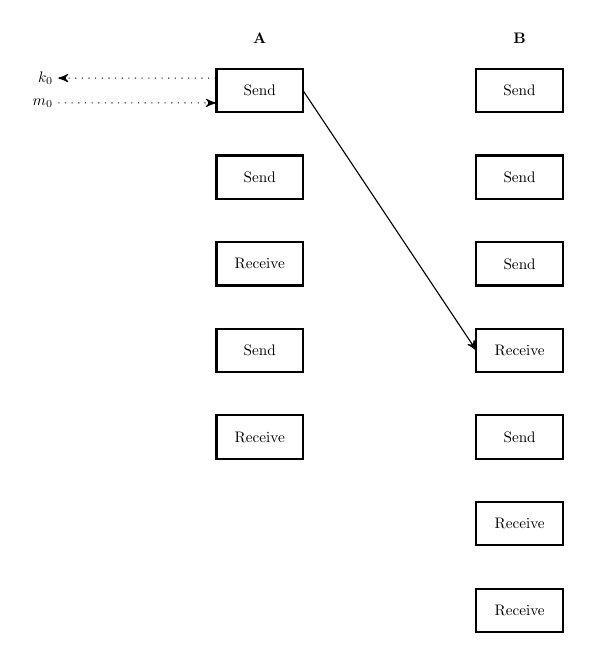
\begin{tikzpicture}[
  box/.style={rectangle,draw,inner sep=5pt,minimum height=1cm,minimum width=2cm,thick},
  node distance=2cm,
  ->,>=stealth',
  scale=0.55, every node/.style={scale=0.55}
]

  % Box t0
  \node [box] (t0) {Send};
  \node [coordinate,right of=t0,node distance=1cm] (tl0) {};
  \node [coordinate,above left=-0.125cm and 0cm of t0,node distance=1cm] (ta0) {};
  \node [left=2cm of ta0] (taa0) {$k_0$};
  \path (ta0) edge[dotted] node [] {} (taa0);
  \node [coordinate,below left=-0.125cm and 0cm of t0,node distance=1cm] (tb0) {};
  \node [left=2cm of tb0] (tbb0) {$m_0$};
  \path (tbb0) edge[dotted] node [] {} (tb0);


  \node [box,below of=t0] (t1) {Send};
  \node [box,below of=t1] (t2) {Receive};
  \node [box,below of=t2] (t3) {Send};
  \node [box,below of=t3] (t4) {Receive};

  \node [box,right of=t0,node distance=6cm] (t5) {Send};
  \node [box,below of=t5] (t6) {Send};
  \node [box,below of=t6] (t7) {Send};
  \node [box,below of=t7] (t8) {Receive};
  \node [box,below of=t8] (t9) {Send};
  \node [box,below of=t9] (t10) {Receive};
  \node [box,below of=t10] (t11) {Receive};

  \node [coordinate,left of=t8,node distance=1cm] (tl8) {};
  \path (tl0) edge[] node [] {} (tl8);

  \node [above=0.25cm of t0] (alice) {\bfseries{A}};
  \node [above=0.25cm of t5] (bob) {\bfseries{B}};
\end{tikzpicture} 
  \caption{Example of Ratcheted Traffic}
  \label{fig:traffic}
\end{figure}
Figure~\ref{fig:traffic} shows an example asynchronous traffic
transcript. The initial states of Alice and Bob are created and
distributed by a trusted party, these states are updated with each
send or receive operation. In the case of a key-agreement protocol the
update information corresponding to the created key of the sender
should generate the same key at the receiver when the update message
is received. Analogous, for a messaging protocol where a encrypted
message should be correctly deciphered by the receiver upon
arrival. In figure for example the message sent by Alice at time $t_0$
is only received by Bob at time $t_8$ but should nonetheless produce a
correct key or plaintext regardless of the messages sent by Bob in the
meantime that updated Bob's state.

\section{Ratchet Security}
\label{sec:ratchet-security}

These continuous updates of the states are supposed to be irreversible
such that past states may not be derived from any future state thus
yielding forward security protecting past messages from being
compromised. This was the original goal that ratcheting tried to
achieve. Naively, a ratchet can be constructed through the usage of a
one-way function the simply updates the states of the communicating
parties. In practice, a hash-function would be deployed as a
reasonable alternative with the downside of losing the asynchronous
communication property~\cite{bellare2003forward}. On the other hand if
some randomness is included in the creation of an updated state we can
protect future states from being recreated by an adversary after an
exposure yielding future secrecy or post-compromise security. Another
way is the usage of some key-agreement protocol to schedule the
creation of new states between the parties~\cite{cohn2016post}.  Again
both constructions come at the cost of losing asynchronous
communications. Asynchronous communications is thus a challenging
obstacle that significantly complicates the design and analysis
of ratcheted key-agreement or messaging protocols.

\bigskip

The adversary in ratcheted protocols is quite powerful and can be both
passive and to a certain extend active. This means he has access to
the full message transcript, can expose the states of both
participants, corrupt the states or impersonate users and in some
cases even choose the randomness used by the participants. As it is
usual in such cases we assess the advantage of any adversary as part
of some key (KIND) or ciphertext (CIND) indistinguishability game
where the adversarial algorithm $\mathcal{A}$ has access to the send
and receive procedures of both Alice and Bob can expose their states
and in the end tries to distinguish some key from random in the KIND
game or decide which one of two chosen messages corresponds to a given
ciphertext in the CIND game.

\begin{figure}[ht]
  \centering
  \setlength{\fboxsep}{10pt}
  \scalebox{0.8}{%
    \fbox{%
      \algrenewcommand\textproc{}
      \algrenewcommand\algorithmicprocedure{\textbf{Game}}

      \begin{minipage}{.5\linewidth}
        \begin{algorithmic}[1]
          \Procedure{$\t{KIND}_b^\mathcal{A}$}{}
          \State $(\t{st}_\t{A},\t{st}_\t{B}) \gets$ \Call{Init}{$1^\lambda$}
          \State $b' \gets \mathcal{A}^{\t{RATCH,EXP,TEST}}$
          \State \Return $b'$
          \EndProcedure
        \end{algorithmic}
      \end{minipage}

      \vline

      \algrenewcommand\textproc{}
      \algrenewcommand\algorithmicprocedure{\textbf{Oracle}}

      \begin{minipage}{.5\linewidth}
        \begin{algorithmic}[1]
          \Procedure{TEST}{$\t{P}$}
          \If{$b = 1$}
          \State \Return $k_\t{P}$
          \EndIf
          \State \Return random $\{0,1\}^{|k_\t{P}|}$ 
          \EndProcedure

          \item[] % Blank line.

          \Procedure{EXP}{$\t{P}$}
          \State \Return $\t{st}_\t{P}$ 
          \EndProcedure
       \end{algorithmic}
     \end{minipage}%
    }
  }
  \caption{Generic Key-Indistinguishability Game}
  \label{fig:kind}
\end{figure}

Figure~\ref{fig:kind} depicts a generic KIND game where \texttt{RATCH} denotes
the send or receive procedures for both Alice and Bob, at will callable by the
adversary. We can similarly define the CIND game in figure~\ref{fig:cind}.

\begin{figure}[ht]
  \centering
  \setlength{\fboxsep}{10pt}
  \scalebox{0.8}{%
    \fbox{%
      \algrenewcommand\textproc{}
      \algrenewcommand\algorithmicprocedure{\textbf{Game}}

      \begin{minipage}{.5\linewidth}
        \begin{algorithmic}[1]
          \Procedure{$\t{CIND}_b^\mathcal{A}$}{}
          \State $(\t{st}_\t{A},\t{st}_\t{B}) \gets$ \Call{Init}{$1^\lambda$}
          \State $b' \gets \mathcal{A}^{\t{RATCH',EXP}}$
          \State \Return $b'$
          \EndProcedure
        \end{algorithmic}
      \end{minipage}

      \vline

      \algrenewcommand\textproc{}
      \algrenewcommand\algorithmicprocedure{\textbf{Oracle}}

      \begin{minipage}{.5\linewidth}
        \begin{algorithmic}[1]
          \Procedure{RATCH'}{$\t{P},m_0,m_1$}
          \State \Return \Call{RATCH}{$\t{P},m_b$}
          \EndProcedure

          \item[] % Blank line.

          \Procedure{EXP}{$\t{P}$}
          \State \Return $\t{st}_\t{P}$ 
          \EndProcedure
       \end{algorithmic}
     \end{minipage}%
    }
  }
  \caption{Generic Ciphertext-Indistinguishability Game}
  \label{fig:cind}
\end{figure}

It is important to note that the way the games are defined is
not sufficient since there exist trivial strategies that make an adversary
succeed. If for example Bob's state is exposed right before he
receives a message then an adversary can easily recover the plaintext
from the message in a messaging protocol or compute the session key
from the message in a key-agreement protocol. It is exactly the
identification of such trivial attacks that pose the greatest
challenge in designing ratcheted protocols implying that the security games
have to be modified to disallow these trivial attacks. Naturally,
the fewer attacks are excluded by the games the securer the overall
protocol becomes. Once the games have been adjusted we can
quantify the advantage of any adversary restricted to some amount queries
and some time complexity as
\[
  \t{Adv}(\mathcal{A}) = \left| \Pr \left[ \t{\{C,K\}IND}_0^\mathcal{A} \rightarrow 1 \right] -
                                \Pr \left[ \t{\{C,K\}IND}_1^\mathcal{A} \rightarrow 1 \right]
                         \right|.
\]



\section{A Brief History of Ratcheted Protocols}
\label{sec:brief-hist-ratch}

As already pointed out the formal analysis of Signal in 2017 marked the
starting point for a slew of ratcheted messaging and key-agreement
protocols. The first protocol was proposed by Bellare et
al.~\cite{bellare2017ratcheted} which established a secure key
exchange protocol for the unidirectional channel that however does not
permit any exposure of the receiver state. Afterwards, Poettering and
Rösler~\cite{poettering2018towards} presented a secure bidirectional
key-agreement protocol in the random oracle model. Around the same
time Jaeger and Stepanovs~\cite{jaeger2018optimal} proposed a similar
messaging protocol. To this date, these two protocols achieve the
highest degree of security at the cost of extremely increased running
times.  Later on Durak and Vaudenay~\cite{durak2018bidirectional}
published an efficient bidirectional key-agreement protocol with minor
concessions in terms of security compared to
\cite{poettering2018towards} and \cite{jaeger2018optimal}.  Next in
the line was a messaging protocol by Jost, Maurer and
Mularczyk~\cite{jostefficient} attempting to close the gap between
\cite{durak2018bidirectional} and
\cite{poettering2018towards,jaeger2018optimal}. It offers a higher
security level than \cite{durak2018bidirectional}, though not reaching
\cite{poettering2018towards,jaeger2018optimal}, but is slower in
comparison. The currently last protocol in the line is a construction
from Alwen, Coretti, and Dodis~\cite{alwen2018double}. It takes
a different approach then the other protocol by building an
improved version of the original Signal protocol instead of
coming up with entirely new algorithms. It is an efficient protocol
that does not quite hold up with the other protocols in terms of
security but is the only one that offers immediate decryption,
the ability to decipher messages even if they arrive in
a different order that than they were initially sent in.
In the following sections we will look more closely into all
above described protocols except~\cite{bellare2017ratcheted}.

\section[Poettering and Rösler]
{Poettering and Rösler~\cite{poettering2018towards}}
\label{sec:poettering-roesler}

This key-agreement protocol was released in the paper
\textit{Asynchronous Ratcheted Key Exchange} in May 2018.
The fact that sets this protocol, and the protocol in the following
section, apart from the others is the notion of \textit{fine-grained}
post-compromise security, meaning that there still remain some
security guarantees concerning the message that directly follows a
state compromise. This kind of security is not supported in
the other protocols where such a message can be fully deciphered
or forged by the adversary. It thus excludes fewer trivial attacks
from their security game, however it does not allow the leakage
or adversarial choice of randomness. The authors conjecture that
fine-grained post-compromise security marks the lower bound
of how many trivial attacks a ratcheted protocol may exclude, hence
the security level achieved in their protocol is optimal.
Surprisingly enough, some heavyweight primitives are required
to reach this lower bound at the cost of an extensive decline
in performance as we will see in the next chapter.

\subsection{Primitives}
\label{sec:primitives}

The protocol proposes a new cryptographic primitive that extends the
functionality of an ordinary key-encapsulation mechanism with an
key update algorithm.
\begin{itemize}
\item \textbf{Key-Updatable Key-Encapsulation Mechanism (ku-KEM).} The primitive
  consists of four procedures, a initial key generation algorithm ($\t{gen}_\t{K}$), an
  key-encapsulation procedure (enc), a corresponding decapsulation procedure (dec) and
  an update procedure for both the public and secret key. Let $\mathcal{PK}$ be
  the public key domain, $\mathcal{SK}$ the secret key domain and $\mathcal{AD}$ the
  associated data domain. We have the following correctness notion, for all
  $(sk_0, pk_0) \in \t{gen}$ and $ad_1,...,ad_n \in \mathcal{AD}$, if
  $sk_i = \t{up}(sk_{i-1},ad_i) \in \mathcal{SK}$ and
  $pk_i = \t{up}(pk_{i-1},ad_i) \in \mathcal{PK}$ for all $i$, then for all
  $(k,c) \in \t{enc}(pk_n)$ we have $\t{dec}(sk_n,c)=k$.
\end{itemize}
In security terms a ku-KEM should satisfy the guarantees of regular
key-encapsulation mechanisms plus some kind of forward security that
protects past keys from state exposures. A ku-KEM can be constructed
out of any hierarchical identity-based encryption scheme
(HIBE)~\cite{gentry2002hierarchical}. Contrary to an ordinate
identity-based encryption scheme where there is a single central
authority handing out secret keys to the users, a HIBE consists
of hierarchical tree structure of many authorities on different levels
such that an authority can access the keys distributed by its children
but its own keys remain inaccessible to any authority on a lower level.
As with ordinary IBE schemes HIBE schemes are usually based on pairing- or
lattice-based cryptography which is far more inefficient than
regular public-key cryptography on elliptic curves.
Next to a HIBE, the protocol requires some other, more standard, primitives.
\begin{itemize}
\item \textbf{One-Time Signature Scheme (OTS).} It consists of three procedures, a initial
  key generation algorithm $\t{gen}_\t{S} \rightarrow \mathcal{SK} \times \mathcal{VK}$,
  a signature algorithm $\t{sgn}: \mathcal{SK} \times \mathcal{M} \rightarrow \Sigma$
  and its corresponding verification algorithm
  $\t{vfy}: \mathcal{VK} \times \mathcal{M} \times \Sigma \rightarrow \{\t{T,F}\}$ with
  $\mathcal{M}$ being the message domain,
  $\mathcal{SK}$ the signing key domain, $\mathcal{VK}$ the verification key domain and
  $\Sigma$ the signature domain.
  We have the following correctness notion, for all $(sgk,vfk) \in \t{gen}_\t{S}$ and
  $m \in \mathcal{M}$ and $\sigma \in \t{sgn}(sgk,m)$ we have $\t{T} = \t{vfy}(vfk,m,\sigma)$.
  We further require strong unforgeability as the security level.
\item \textbf{Random Oracle}. As the protocol is secure in the random oracle H it demands
  a random oracle function H. In practice, H is replaced by a standard hash function.
\end{itemize}

\subsection{Construction}
\label{sec:construction}

Poettering and Rösler give three separate constructions in their article.
A unidirectional protocol (URKE), a sesquidirectional construction (SRKE) in which
Bob can reply without establishing a key, finally both URKE and SRKE
are used to create a bidirectional asynchronous key-exchange protocol (BRKE)
with optimal security. The construction is quite involved with long
procedures, figure~\ref{fig:brke} prunes out some parts not necessary for the
analysis of the benchmarks in the next chapter.

% TODO: Complete algorithm.

\begin{figure}[H]
  \centering
  \setlength{\fboxsep}{10pt}
  \scalebox{0.9}{%
    \fbox{%
      \algrenewcommand\textproc{}
      \algrenewcommand\algorithmicprocedure{\textbf{func}}

      \begin{minipage}{.5\linewidth}
        \begin{algorithmic}[1]
          \Procedure{init}{}
          \For{$u \in \{A,B\}$}
            \State $(sgk_u, vfk_u) \gets \t{gen}_\t{S}$
            \State $(sk_u, pk_u) \gets \t{gen}_\t{K}$
            \State random $K_u \in \{0,1\}^{|\mathcal{K}|}$
            \State $(E^\vdash,E^\dashv) \gets 0; \ (s,r) \gets 0$
            \State $PK_u[0] \gets pk_u; \ SK_u[0] \gets sk_u$
            \State $S_u \gets (PK_{\bar{u}},E,s,vfk_{\bar{u}},K_{\bar{u}})$
            \State $R_u \gets (SK_u,E,r,sgk_u,K_u)$
            \State $ST_u \gets (R_u,S_u)$
          \EndFor
          \State \Return $(ST_A,ST_B)$
          \EndProcedure
        \end{algorithmic}
      \end{minipage}

      \vline

      \algrenewcommand\textproc{}
      \algrenewcommand\algorithmicprocedure{\textbf{Oracle}}

      \begin{minipage}{.5\linewidth}
        \begin{algorithmic}[1]
          \Procedure{RATCH'}{$\t{P},m_0,m_1$}
          \State \Return \Call{RATCH}{$\t{P},m_b$}
          \EndProcedure

          \item[] % Blank line.

          \Procedure{EXP}{$\t{P}$}
          \State \Return $\t{st}_\t{P}$ 
          \EndProcedure
       \end{algorithmic}
     \end{minipage}%
    }
  }
  \caption{Bidirectional Asynchronous Key-Exchange Protocol (BRKE)}
  \label{fig:brke}
\end{figure}

An important concept in the above protocols is the notion epochs
controlled by the $E_S^\vdash,E_S^\dashv$ and $E_R^\vdash,E_R^\dashv$
variables in the state of each user. They basically determine
the complexity of the send and receive procedures due to their
control of the loop bounds.

% TODO Explain epochs.

\section[Jaeger and Stepanovs]{Jaeger and Stepanovs~\cite{jaeger2018optimal}}
\label{sec:jaeger-stepanovs}

This secure messaging protocol was published in the paper
\textit{Optimal Channel Security Against Fine-Grained State Compromise: The Safety of Messaging}
in June 2018 and targets similar a security level as the protocol by
Poettering and Rösler although aiming at secure communication instead
of key-exchange and with considering the leakage of randomness.

\subsection{Primitives}
\label{sec:primitives-1}

The protocol, again as in the Poettering and Rösler case, uses a HIBE to construct
one of two novel primitives.
\begin{itemize}
\item \textbf{Key-Updatable Public-Key Encryption Scheme (ku-PKE).} The primitive
  consists of five routines. A key generation algorithm
  $\t{PKE.Kg} \rightarrow \mathcal{DK} \times \mathcal{EK}$, an encryption
  procedure $\t{PKE.Enc}: \mathcal{EK} \times \mathcal{M} \rightarrow \mathcal{C}$,
  a corresponding decryption function
  $\t{PKE.Dec}: \mathcal{DK} \times \mathcal{C} \rightarrow \mathcal{M}$ and
  a public-key and private-key update algorithms
  $\t{PKE.UpdEk}: \mathcal{EK} \times \Delta \rightarrow \mathcal{EK}$,
  $\t{PKE.UpdDk}: \mathcal{DK} \times \Delta \rightarrow \mathcal{DK}$, where
  $\mathcal{EK}$ denotes the encryption key domain, $\mathcal{DK}$ the
  decryption key domain, $\mathcal{M}, \mathcal{C}$ the message and
  ciphertext domain respectively. We have the following correctness notion, for all
  $(dk_0, ek_0) \in \t{gen}$ and $\delta_1,...,\delta_n \in \Delta$, if
  $dk_i = \t{PKE.UpdDk}(dk_{i-1},\delta_i)$ and
  $ek_i = \t{PKE.UpdEk}(ek_{i-1},\delta_i)$ for all $i$, then for all
  $c \in \t{enc}(ek_n,m)$ we have $\t{dec}(dk_n,c)=m$.
\end{itemize}

The construction of a ku-PKE is trivially performed out of a HIBE thus if
the HIBE is IND-CCA secure so is the ku-PKE. Furthermore, as with the
ku-KEM, we expect forward security in the case of exposures.
Jaeger and Stepanovs define a second novel primitive for use in the final protocol.
\begin{itemize}
\item \textbf{Key-Updatable Digital Signature Scheme (ku-DSS).} The primitive
  consists of five routines. A key generation algorithm
  $\t{DSS.Kg} \rightarrow \mathcal{SK} \times \mathcal{VK}$, a signing routine
  $\t{DSS.Sign}: \mathcal{SK} \times \mathcal{M} \rightarrow \Sigma$, its
  corresponding verification function
  $\t{DSS.Vrfy}: \mathcal{VK} \times \mathcal{M} \times \Sigma \rightarrow \{\t{T,F}\}$ and
  two public/private-key update routines
  $\t{DSS.UpdVk}: \mathcal{VK} \times \Delta \rightarrow \mathcal{VK}$ and
  $\t{DSS.UpdSk}: \mathcal{SK} \times \Delta \rightarrow \mathcal{SK}$, where
  $\mathcal{VK}$ is the signing key domain, $\mathcal{SK}$ the verification key
  domain and $\mathcal{M}, \Sigma$ are the message and signature domains.
\end{itemize}

In order to construct a ku-DSS we need a forward-secure signature scheme. As
security level we require unforgeability as well as forward-secrecy under
exposures. 

\subsection{Construction}
\label{sec:construction-1}

Figure contains the full secure channel protocol (SCh) based on a collision-resistant
hash function H, a key-updatable public-key encryption scheme PKE and
a key-updatable digital signature scheme.

% TODO: Complete algorithm.

\begin{figure}[H]
  \centering
  \setlength{\fboxsep}{10pt}
  \scalebox{0.9}{%
    \fbox{%
      \algrenewcommand\textproc{}
      \algrenewcommand\algorithmicprocedure{\textbf{func}}

      \begin{minipage}{.5\linewidth}
        \begin{algorithmic}[1]
          \Procedure{init}{}
          \For{$u \in \{A,B\}$}
            \State $(sgk_u, vfk_u) \gets \t{gen}_\t{S}$
            \State $(sk_u, pk_u) \gets \t{gen}_\t{K}$
            \State random $K_u \in \{0,1\}^{|\mathcal{K}|}$
            \State $(E^\vdash,E^\dashv) \gets 0; \ (s,r) \gets 0$
            \State $PK_u[0] \gets pk_u; \ SK_u[0] \gets sk_u$
            \State $S_u \gets (PK_{\bar{u}},E,s,vfk_{\bar{u}},K_{\bar{u}})$
            \State $R_u \gets (SK_u,E,r,sgk_u,K_u)$
            \State $ST_u \gets (R_u,S_u)$
          \EndFor
          \State \Return $(ST_A,ST_B)$
          \EndProcedure
        \end{algorithmic}
      \end{minipage}

      \vline

      \algrenewcommand\textproc{}
      \algrenewcommand\algorithmicprocedure{\textbf{Oracle}}

      \begin{minipage}{.5\linewidth}
        \begin{algorithmic}[1]
          \Procedure{RATCH'}{$\t{P},m_0,m_1$}
          \State \Return \Call{RATCH}{$\t{P},m_b$}
          \EndProcedure

          \item[] % Blank line.

          \Procedure{EXP}{$\t{P}$}
          \State \Return $\t{st}_\t{P}$ 
          \EndProcedure
       \end{algorithmic}
     \end{minipage}%
    }
  }
  \caption{Secure Channel Protocol (SCh)}
  \label{fig:secure-channel}
\end{figure}

\section[Durak and Vaudenay]
{Durak and Vaudenay~\cite{durak2018bidirectional}}
\label{sec:durak-vaudenay}

This key-agreement protocol was published in the paper
\textit{Bidirectional Asynchronous Ratcheted Key Agreement without
Key-Update Primitives}, short BARK, in September 2018. It was the first approach to
create a simple but efficient protocol without the use of slow,
hand-tailored primitives at the cost of not supporting fine-grained
post-compromise security. Furthermore, the protocol explicitly spells
out the trivial attacks, although disallowing more than the previous
two protocols, and bundles them in form a \textit{cleanness-predicate}
which greatly simplifies the security games and its accompanying
security proofs. The authors also introduce a new notion called
recover security stating that if one participant is compromised he
looses authenticity for a short while in which an adversary can
impersonate the victim until he recovers from the leakage. Clearly, if
the victim simply recovers from the exposure both the participants may
never detect that there was an active impersonation attack in place,
the protocol thus advocates to detect such forgeries right after a
state exposure and immediately cut the communication as a
consequence. Such recover security can easily be achieved with a
collision resistant hash function that chain hashes the entire
communication transcript. As the cherry on cake the papers shows that
a weaker unidirectional version of the protocol already implies
public-key cryptography which essentially shatters any hopes of
achieving similar levels of security with symmetric primitives.

\subsection{Primitives}
\label{sec:primitives-2}

As already indicated the protocol does not deploy any intricate
cryptographic primitives. Next to the hash function combines a
public-key encryption scheme and a digital signature scheme to
a signcryption algorithm.
\begin{itemize}
\item \textbf{Signcryption Scheme (SC).} This primitive consists of four routines,
  two key generation algorithms one creating the PKE keys
  $\t{Gen}_\t{R} \rightarrow \mathcal{SK}_\t{R} \times \mathcal{PK}_\t{R}$ and
  similarly for the creation of the DSS keys
  $\t{Gen}_\t{S} \rightarrow \mathcal{SK}_\t{S} \times \mathcal{PK}_\t{S}$ where
  $(\mathcal{PK}_\t{R},\mathcal{SK}_\t{R})$ are the PKE key domains and
  $(\mathcal{PK}_\t{S},\mathcal{SK}_\t{S})$ are the DSS key domains. Furthermore,
  there is an encryption procedure
  $\t{Enc}: \mathcal{SK}_\t{S} \times \mathcal{PK}_\t{R} \times
   \rightarrow \mathcal{C}$ and its corresponding
  decryption function
  $\t{Dec}: \mathcal{SK}_\t{R} \times \mathcal{PK}_\t{S}
  \mathcal{C} \times \mathcal{AD} \rightarrow \mathcal{M}$ with $\mathcal{AD}$
  being the associated data domain and $(\mathcal{M}, \mathcal{C})$ being
  the message and ciphertext domain respectively. We have the following
  correctness notion, for all $m \in \mathcal{M}$, $ad \in \mathcal{AD}$,
  $(sk_R,pk_R) \in \t{Gen}_\t{R}$ and $(sk_S,pk_S) \in \t{Gen}_\t{S}$ it
  holds that $\t{Dec}(sk_R,pk_S,ad,\t{Enc}(sk_S,pk_R,ad,m)) = m$.
\end{itemize}

A signcryption scheme can be constructed by naively chaining a DSS and PKE scheme
such that $\t{Enc}(sk_S,pk_R,ad,m) = \t{PKE.Enc}(pk_R,m || \t{DSS.Sign}(sk_S,ad || m))$.
The BARK protocol demands that the PKE cryptosystem is IND-CCA secure and the
DSS scheme is EF-OTCMA secure.

\subsection{Construction}
\label{sec:construction-2}

Similar to the protocol by Poettering and Rösler the BARK protocol is
constructed via a smaller unidirectional protocol. Figure~\ref{fig:uni-arcad}
shows the unidirectional ARCAD messaging protocol that is KIND-secure but
does not offer recover security. The composition of two uniARCAD yields
the full BARK protocol as shown in figure~\ref{fig:bark}

\begin{figure}[ht]
  \centering
  \setlength{\fboxsep}{10pt}
  \scalebox{0.9}{%
    \fbox{%
      \algrenewcommand\textproc{}
      \algrenewcommand\algorithmicprocedure{\textbf{func}}

      \begin{minipage}{.5\linewidth}
        \begin{algorithmic}[1]
          \Procedure{uniARCAD.Init}{$1^\lambda$}
          \State $(\t{sk}_\t{S},\t{pk}_\t{S}) \gets$ \Call{$\t{Gen}_\t{S}$}{$1^\lambda$}
          \State $(\t{sk}_\t{R},\t{pk}_\t{R}) \gets$ \Call{$\t{Gen}_\t{R}$}{$1^\lambda$}

          \State $\t{st}_\t{S} \gets (\t{sk}_\t{S},\t{pk}_\t{R})$ 
          \State $\t{st}_\t{S} \gets (\t{sk}_\t{R},\t{pk}_\t{S})$ 

          \State \Return $(\t{st}_\t{S},\t{st}_\t{R})$
          \EndProcedure

          \item[]

          \Procedure{uniARCAD.Receive}{$\t{st}_\t{R}, \t{ad}, \t{ct}$}
          \State $(\t{sk}_\t{R},\t{pk}_\t{S}) \gets \t{st}_\t{R}$ 
          \State $\t{pt}' \gets$ \Call{Dec}{$\t{sk}_\t{R},\t{pk}_\t{S},\t{ad},\t{ct}$}
          \If{$\t{pt}' = \perp$}
          \State \Return $(\t{false}, \t{st}_\t{R}, \perp)$
          \EndIf
          \State $(\t{pt},\t{st}_\t{R}') \gets \t{pt}'$
          \State \Return $(\t{true},\t{st}_\t{R}, \t{pt})$
          \EndProcedure
         
        \end{algorithmic}
      \end{minipage}

      \begin{minipage}{.5\linewidth}
        \begin{algorithmic}[1]
          \Procedure{uniARCAD.Send}{$\t{st}_\t{S}, \t{ad}, \t{pt}, \t{flag}$}
          \State $(\t{sk}_\t{S},\t{pk}_\t{R}) \gets \t{st}_\t{S}$ 
          \If{$\t{flag} = \t{true}$}
          \State $(\t{sk}_\t{S}',\t{pk}_\t{S}') \gets$ \Call{SC.Gen}{$1^\lambda$}
          \State $(\t{sk}_\t{R}',\t{pk}_\t{R}') \gets$ \Call{SC.Gen}{$1^\lambda$}
          \State $\t{st}_\t{S}' \gets (\t{sk}_\t{S}',\t{pk}_\t{R}')$
          \State $\t{st}_\t{R}' \gets (\t{sk}_\t{R}',\t{pk}_\t{S}')$
          \Else
          \State $(\t{sk}_\t{S}',\t{pk}_\t{R}') \gets (\perp,\perp)$
          \EndIf
          \State $\t{pt}' \gets (\t{st}_\t{R}', \t{pt})$
          \State $\t{ct} \gets$ \Call{Enc}{$\t{sk}_\t{S},\t{pk}_\t{R}, \t{ad}, \t{pt}'$}
          \State \Return $(\t{st}_\t{S}', \t{ct})$
          \EndProcedure
          
        \end{algorithmic}
      \end{minipage}%
    }
  }
  \caption{Unidirectional ARCAD Protocol}
  \label{fig:uni-arcad}
\end{figure}

Contrarily to the other protocols BARK is quite self-explanatory. It
operates on the basis of onion encryptions where repeated unidirectional
traffic builds up an chain of receiving states that have to traversed once
a response is received since the outgoing messages contained
the sender states which are used to encrypt said response.
Also note that the creation of new sending and receiving states
is not necessary in but the inner most layer of the onion hence
there is a flag passed to \texttt{uniARCAD.Send}. The
\texttt{HSent} and \texttt{HReceived} chain-hash variables
ensure the recover security.

\begin{figure}[H]
  \centering
  \setlength{\fboxsep}{10pt}
  \scalebox{0.9}{%
    \fbox{%
      \algrenewcommand\textproc{}
      \algrenewcommand\algorithmicprocedure{\textbf{func}}

      \begin{minipage}{\linewidth}
        \begin{algorithmic}[1]
          \Procedure{BARK.Init}{$1^\lambda$}
          \State $(\t{st}_\t{A,send},\t{st}_\t{B,rec}) \gets$ \Call{uniBARK.Init}{$1^\lambda$}
          \State $(\t{st}_\t{B,send},\t{st}_\t{A,rec}) \gets$ \Call{uniBARK.Init}{$1^\lambda$}
          \State $\t{hk} \gets$ \Call{H.Init}{$1^\lambda$}
          \State $\t{st}_\t{A} \gets (\t{hk}, \t{st}_\t{A,send}, \t{st}_\t{A,rec},
          \perp, \perp, 0, 10)$ 
          \State $\t{st}_\t{B} \gets (\t{hk}, \t{st}_\t{B,send}, \t{st}_\t{B,rec},
          \perp, \perp, 0, 10)$
          \State \Return $(\t{st}_\t{A},\t{st}_\t{B})$
          \EndProcedure
          
          \item[]
          
          \Procedure{BARK.Send}{$\t{st}_\t{P}, \t{ad}, \t{pt}$}
          \State $(\t{hk}, \t{st}_\t{P,send}, \t{st}_\t{P,rec},
          \t{Hsent}, \t{Hreceived}, \t{rt}, \t{rt}_\t{max}) \gets \t{st}_\t{P}$
          
          \If{$\t{rt} = \t{rt}_\t{max}$}
          \State $(\t{st}_\t{S,new}, \t{st}_\t{P,rec}) \gets$
          \Call{uniBARK.Init}{$1^\lambda$}
          \State $\t{msg} \gets (\t{st}_\t{S,new}, \t{pt})$
          \Else
          \State $\t{msg} \gets (\perp, \t{pt})$
          \EndIf
          \State $(\t{st}_\t{P,send}, \t{ct'}) \gets$
          \Call{uniBARK.Send}{$\t{st}_\t{P,send}, \t{ad}, \t{msg}, \t{rt} = \t{rt}_\t{max}$}
         
          \State $\t{ct} \gets (\t{Hsent}, \t{ct'}, \t{rt}_\t{S} = \t{rt}_\t{max})$ 
          \State $\t{Hsent} \gets$ \Call{H.Eval}{$\t{hk}, (\t{ad}, \t{ct})$}
          
          \State $\t{st}_\t{P} \gets (\t{hk}, \t{st}_\t{P,send}, \t{st}_\t{P,rec},
          \t{Hsent}, \t{Hreceived}, \t{rt} + 1 \mod \t{rt}_\t{max}, \t{rt}_\t{max})$
          \State \Return $(\t{st}_\t{P}, \t{ct})$
          \EndProcedure
          
          \item[] % blank line
          
          \Procedure{BARK.Receive}{$\t{st}_\t{P}, \t{ad}, \t{ct}$}
          \State $(\t{hk}, \t{st}_\t{P,send}, \t{st}_\t{P,rec},
          \t{Hsent}, \t{Hreceived}, \t{rt}, \t{rt}_\t{max}) \gets \t{st}_\t{P}$
          \State $(\t{h}, \t{ct'}, \t{rt}_\t{S}) \gets \t{ct}$
          \If{$\t{Hreceived} \neq \t{h}$} \State \Return $(\t{false}, \t{st}_\t{P})$
          \EndIf
          
          \State $(\t{acc}, \t{st}_\t{P,rec}, \t{msg}) \gets$
          \Call{uniBARK.Receive}{$\t{st}_\t{P,rec}, \t{ad}, \t{ct'}, \t{rt}_\t{S} =
          \t{rt}_\t{max}$}
          \If{$\t{acc} = \t{false}$} \State \Return $(\t{false}, \t{st}_\t{P})$ \EndIf
          
          \If{$\t{rt}_\t{S} = \t{rt}_\t{max}$}
          \State $(\t{st}_\t{P,send}, \t{pt}) \gets \t{msg}$
          \Else
          \State $(\perp, \t{pt}) \gets \t{msg}$
          \EndIf
          
          \State $\t{Hreceived} \gets$ \Call{H.Eval}{$\t{hk}, (\t{ad}, \t{ct})$}
          
          \State $\t{st}_\t{P} \gets (\t{hk}, \t{st}_\t{P,send}, \t{st}_\t{P,rec},
          \t{Hsent}, \t{Hreceived}, \t{rt}, \t{rt}_\t{max})$
          \State \Return $(\t{true}, \t{st}_\t{P}, \t{pt})$
          \EndProcedure
        \end{algorithmic}
      \end{minipage}
    } 
  }
  \caption{BARK Protocol}
  \label{fig:bark}
\end{figure}

\section[Jost, Maurer and Mularczyk]
{Jost, Maurer and Mularczyk~\cite{jostefficient}}
\label{sec:jost-maur-mularczyk}

This secure messaging protocol was published in the paper
\textit{Efficient Ratcheting: Almost-Optimal Guarantees for Secure Messaging}
in early October 2018. It offers near-optimal security guarantees similar
to the protocols by Poettering, Rösler and Jaeger, Stepanovs while
deploying lighter primitives than the latter two. Effectively, the protocol
only excludes some special cases of fine-grained post-compromise security
thus offering a slightly higher security level than the protocol by
Durak and Vaudenay. It also decouples the leakage of random coins
from state exposures with all security proofs being in the random
oracle model.

\subsection{Primitives}
\label{sec:primitives-3}

The protocol proposes several novel cryptographic primitives that can all be
mounted by regular public-key key cryptosystems to extend them
with key-update routines.
\begin{itemize}
\item \textbf{Key-Updating Signature (KuSig).} This primitive consists of
  three routines. A key generation algorithm
  $\t{Gen} \rightarrow \mathcal{VK} \times \mathcal{SK}$, a signing function
  $\t{Sign}: \mathcal{SK} \times \mathcal{M} \rightarrow \mathcal{SK} \times \Sigma$
  and its corresponding verification procedure
  $\t{Ver}: \mathcal{VK} \times \mathcal{M} \times \Sigma
  \rightarrow \mathcal{VK} \times \{\t{T,F}\}$
  where $\mathcal{VK}$ is the verification key domain, $\mathcal{SK}$ the signing
  key domain and $\mathcal{M},\Sigma$ are the message and the signature domains
  respectively. We have the following correctness notion,
  if $(\t{vk}_0,\t{sk}_0) \leftarrow \t{Gen}$ then for any sequence of
  messages $m_1,...,m_k \in \mathcal{M}$ and for all $i \in [k]$
  such that $(\t{sk}_i,\sigma_i) \leftarrow \t{Sign}(\t{sk}_{i-1},m_i)$
  and $(\t{vk}_i,v_i) \leftarrow \t{Ver}(\t{vk}_{i-1},\sigma_i)$ we have
  that $v_i = \t{T}$.
\end{itemize}

As the security level we require resistance against universal forgeries
with added forward security in case of state exposures.

\begin{itemize}
\item \textbf{Secretly Key-Updatable Public-Key Encryption (SkuPke).} This
  primitive consists of six routines. A key generation algorithm
  $\t{Gen} \rightarrow \mathcal{EK} \times \mathcal{DK}$, an encryption
  routine $\t{Enc}: \mathcal{EK} \times \mathcal{M} \rightarrow \mathcal{C}$ and
  its corresponding decryption function
  $\t{Dec}: \mathcal{DK} \times \mathcal{C} \rightarrow \mathcal{M}$, where
  $\mathcal{EK},\mathcal{DK}$ denote the encryption/decryption key domains
  and $\mathcal{M},\mathcal{C}$ denote the message/ciphertext domains.
  Furthermore, there is an algorithm that generates key update information
  $\t{UpdateGen} \rightarrow \mathcal{UE} \times \mathcal{UD}$ with
  $\mathcal{UE}$ being the public key update information domain and
  $\mathcal{UD}$ being the secret key update information. This two
  arguments can be fed into an encryption key update function
  $\t{UpdateEk}: \mathcal{UE} \times \mathcal{EK} \rightarrow \mathcal{EK}$
  and the respective decryption key update function
  $\t{UpdateDk}: \mathcal{UD} \times \mathcal{DK} \rightarrow \mathcal{DK}$.
  We have the following correctness notion. If $(\t{ek}_0,\t{dk}_0) \in \t{Gen}$ and
  $(\t{ue}_1,\t{ud}_1),...,(\t{ue}_k,\t{ud}_k) \in \t{UpdateGen}$ then
  for all $i \in [k]$ with $\t{ek}_i = \t{UpdateEk}(\t{ue}_i, \t{ek}_{i-1})$ and
  $\t{dk}_i = \t{UpdateDk}(\t{ud}_i, \t{dk}_{i-1})$ and all $m \in \mathcal{M}$
  it holds that $\t{Dec}(\t{dk}_i,\t{Enc}(\t{ek}_i, m)) = m$.
\end{itemize}

The intuition behind this primitive is that the key pair can be
updated independently with update information not linked to any
key where the update information for the encryption key can be freely
exposed while the update information for the decryption should
remain hidden and only change hands through a back-channel.
This scheme can be constructed out of a vanilla components
of the ElGamal cryptosystem. The SkuPke scheme serves to
create another primitive.
\begin{itemize}
\item \textbf{Healable And Key-Updating Public-Key Encryption (HkuPke).} This
  primitive consists of five routines. A key generation algorithm
  $\t{Gen} \rightarrow \mathcal{EK} \times \mathcal{DK}$ and encryption/decryption
  functions
  $\t{Enc}: \mathcal{EK} \times \mathcal{M} \times \mathcal{AD} \rightarrow \mathcal{C}$,
  $\t{Dec}: \mathcal{DK} \times \mathcal{C} \times \mathcal{AD} \rightarrow \mathcal{M}$
  with $\mathcal{EK}$ being the encryption key domain, $\mathcal{DK}$ the decryption
  key domain and $\mathcal{M},\mathcal{C},\mathcal{AD}$ are the message, ciphertext
  and associated data domains. The scheme is completed with two key update
  functions $\t{BcUpEk}: \mathcal{EK} \times \Delta \rightarrow \mathcal{EK}$ and
  $\t{BcUpDk}: \mathcal{DK} \times \Delta \rightarrow \mathcal{DK}$ with
  $\Delta$ being the update information domain.
\end{itemize}

The purpose of the HkuPke scheme is similar to the SkuPke scheme with the difference
that we now still allow the decryption of message for any arbitrary sequence
of \texttt{BcUpDk} calls where only a prefix of the used update information
has been used in \texttt{BcUpEk} calls. The receiver can thus
instigate key updates via a back-channel to start the healing process.

\subsection{Construction}
\label{sec:construction-3}

\begin{figure}[ht]
  \centering
  \setlength{\fboxsep}{10pt}
  \scalebox{0.9}{%
    \fbox{%
      \algrenewcommand\textproc{}
      \algrenewcommand\algorithmicprocedure{\textbf{func}}
      \begin{minipage}{\linewidth}
        {\fontsize{8}{10}\selectfont
        \begin{algorithmic}[1]
          \Procedure{BARK.Init}{$1^\lambda$}
          \State $(\t{st}_\t{A,send},\t{st}_\t{B,rec}) \gets$ \Call{uniBARK.Init}{$1^\lambda$}
          \State $(\t{st}_\t{B,send},\t{st}_\t{A,rec}) \gets$ \Call{uniBARK.Init}{$1^\lambda$}
          \State $\t{hk} \gets$ \Call{H.Init}{$1^\lambda$}
          \State $\t{st}_\t{A} \gets (\t{hk}, \t{st}_\t{A,send}, \t{st}_\t{A,rec},
          \perp, \perp, 0, 10)$ 
          \State $\t{st}_\t{B} \gets (\t{hk}, \t{st}_\t{B,send}, \t{st}_\t{B,rec},
          \perp, \perp, 0, 10)$
          \State \Return $(\t{st}_\t{A},\t{st}_\t{B})$
          \EndProcedure
          
          \item[]
          
          \Procedure{BARK.Send}{$\t{st}_\t{P}, \t{ad}, \t{pt}$}
          \State $(\t{hk}, \t{st}_\t{P,send}, \t{st}_\t{P,rec},
          \t{Hsent}, \t{Hreceived}, \t{rt}, \t{rt}_\t{max}) \gets \t{st}_\t{P}$
          
          \If{$\t{rt} = \t{rt}_\t{max}$}
          \State $(\t{st}_\t{S,new}, \t{st}_\t{P,rec}) \gets$
          \Call{uniBARK.Init}{$1^\lambda$}
          \State $\t{msg} \gets (\t{st}_\t{S,new}, \t{pt})$
          \Else
          \State $\t{msg} \gets (\perp, \t{pt})$
          \EndIf
          \State $(\t{st}_\t{P,send}, \t{ct'}) \gets$
          \Call{uniBARK.Send}{$\t{st}_\t{P,send}, \t{ad}, \t{msg}, \t{rt} = \t{rt}_\t{max}$}
         
          \State $\t{ct} \gets (\t{Hsent}, \t{ct'}, \t{rt}_\t{S} = \t{rt}_\t{max})$ 
          \State $\t{Hsent} \gets$ \Call{H.Eval}{$\t{hk}, (\t{ad}, \t{ct})$}
          
          \State $\t{st}_\t{P} \gets (\t{hk}, \t{st}_\t{P,send}, \t{st}_\t{P,rec},
          \t{Hsent}, \t{Hreceived}, \t{rt} + 1 \mod \t{rt}_\t{max}, \t{rt}_\t{max})$
          \State \Return $(\t{st}_\t{P}, \t{ct})$
          \EndProcedure
          
          \item[] % blank line
          
          \Procedure{BARK.Receive}{$\t{st}_\t{P}, \t{ad}, \t{ct}$}
          \State $(\t{hk}, \t{st}_\t{P,send}, \t{st}_\t{P,rec},
          \t{Hsent}, \t{Hreceived}, \t{rt}, \t{rt}_\t{max}) \gets \t{st}_\t{P}$
          \State $(\t{h}, \t{ct'}, \t{rt}_\t{S}) \gets \t{ct}$
          \If{$\t{Hreceived} \neq \t{h}$} \State \Return $(\t{false}, \t{st}_\t{P})$
          \EndIf
          
          \State $(\t{acc}, \t{st}_\t{P,rec}, \t{msg}) \gets$
          \Call{uniBARK.Receive}{$\t{st}_\t{P,rec}, \t{ad}, \t{ct'}, \t{rt}_\t{S} =
          \t{rt}_\t{max}$}
          \If{$\t{acc} = \t{false}$} \State \Return $(\t{false}, \t{st}_\t{P})$ \EndIf
          
          \If{$\t{rt}_\t{S} = \t{rt}_\t{max}$}
          \State $(\t{st}_\t{P,send}, \t{pt}) \gets \t{msg}$
          \Else
          \State $(\perp, \t{pt}) \gets \t{msg}$
          \EndIf
          
          \State $\t{Hreceived} \gets$ \Call{H.Eval}{$\t{hk}, (\t{ad}, \t{ct})$}
          
          \State $\t{st}_\t{P} \gets (\t{hk}, \t{st}_\t{P,send}, \t{st}_\t{P,rec},
          \t{Hsent}, \t{Hreceived}, \t{rt}, \t{rt}_\t{max})$
          \State \Return $(\t{true}, \t{st}_\t{P}, \t{pt})$
          \EndProcedure
        \end{algorithmic}
        }
      \end{minipage}
    } 
  }
  \caption{Secure Messaging Protocol}
  \label{fig:secmsg}
\end{figure}

\section{Alwen, Coretti and Dodis}
\label{sec:alwen-coretti-dodis}



\chapter{Benchmarks}
\label{chap:benchmarks}

\chapter{On-Demand BARK}
\label{chap:bark}

\chapter{Conclusion}
\label{chap:conclusion}


\bibliographystyle{plainurl}
\bibliography{bibliography}

\listoffigures

\end{document}
